\section{Introduction}

In this chapter, we explore the performance influence of low level
tuning parameters on the performance of SkelCL stencils. We describe
an experiment to enumerate a large optimisation space of Stencil
codes, measuring the relative performance achieved by varying the
workgroup size of OpenCL kernels.


\section{Grid Decomposition in Stencil Codes}

\TODO{Add diagram showing workgroup decomposition.}


\section{Experimental Setup}

% A. Georges, D. Buytaert, and L. Eeckhout, “Statistically Rigorous
% Java Performance Evaluation,” in Proceedings of the 22Nd Annual ACM
% SIGPLAN Conference on Object-oriented Programming Systems and
% Applications, 2007, vol. 42, no. 10, p. 57.
\TODO{%
  Statistically rigorous performance evaluations.~\cite{Georges2007}.
}

\begin{table}
\footnotesize
\centering
\begin{tabular}{| L{7.5cm} | L{1.5cm} | L{1.5cm} | L{1.5cm} | L{1.5cm} | L{1.5cm} |}
\hline
\scriptsize
\centering
\rowcolors{2}{white}{gray!25}
\begin{tabular}{ L{4.5cm} L{1.5cm} L{1.5cm} L{1.5cm} L{1.5cm} L{1.5cm} }
\hline
\scriptsize
\centering
\rowcolors{2}{white}{gray!25}
\begin{tabular}{ L{4.5cm} L{1.5cm} L{1.5cm} L{1.5cm} L{1.5cm} L{1.5cm} }
\hline
\scriptsize
\centering
\rowcolors{2}{white}{gray!25}
\begin{tabular}{ L{4.5cm} L{1.5cm} L{1.5cm} L{1.5cm} L{1.5cm} L{1.5cm} }
\hline
\input{gen/tables/devices}
\hline
\end{tabular}

\hline
\end{tabular}

\hline
\end{tabular}

\hline
\end{tabular}
\caption{%
  Execution devices. \FIXME{Missing data from CPUs!}%
}
\label{tab:hw}
\end{table}

\begin{table}
\footnotesize
\centering
\begin{tabular}{| l | l | l | l | l | l |}
\hline
\scriptsize
\centering
\rowcolors{2}{white}{gray!25}
\begin{tabular}{lrrrrr}
\toprule
      Name &  North &  South &  East &  West &  Instruction Count \\
\midrule
   % complex &     30 &     30 &    30 &    30 &                161 \\
   % complex &      1 &     10 &    30 &    30 &                681 \\
   % complex &     20 &     10 &    20 &    10 &                161 \\
   % complex &      5 &      5 &     5 &     5 &                734 \\
   % complex &      5 &      5 &     5 &     5 &                161 \\
   % complex &      1 &     10 &    30 &    30 &                154 \\
   % complex &     10 &     10 &    10 &    10 &                161 \\
   % complex &     20 &     20 &    20 &    20 &                706 \\
   % complex &      1 &      1 &     1 &     1 &                137 \\
   % complex &     20 &     10 &    20 &    10 &                706 \\
   % complex &      1 &      1 &     1 &     1 &                661 \\
   % complex &     10 &     10 &    10 &    10 &                794 \\
   % complex &     30 &     30 &    30 &    30 &                706 \\
   % complex &     20 &     20 &    20 &    20 &                161 \\
   %  simple &      5 &      5 &     5 &     5 &                 67 \\
   %  simple &     20 &     10 &    20 &    10 &                612 \\
   %  simple &     20 &     20 &    20 &    20 &                612 \\
   %  simple &      1 &     10 &    30 &    30 &                592 \\
   %  simple &     10 &     10 &    10 &    10 &                700 \\
   %  simple &     30 &     30 &    30 &    30 &                612 \\
   %  simple &      1 &      1 &     1 &     1 &                 93 \\
   %  simple &     30 &     30 &    30 &    30 &                 67 \\
   %  simple &     20 &     10 &    20 &    10 &                 67 \\
   %  simple &      5 &      5 &     5 &     5 &                640 \\
   %  simple &     20 &     20 &    20 &    20 &                 67 \\
   %  simple &     10 &     10 &    10 &    10 &                 67 \\
   %  simple &      0 &      0 &     0 &     0 &                 40 \\
   %  simple &      1 &     10 &    30 &    30 &                 65 \\
   %  simple &      1 &      1 &     1 &     1 &                617 \\
   synthetic & 1--30 & 1--30 & 1--30 & 1--30 & 67--137\\
   synthetic & 1--30 & 1--30 & 1--30 & 1--30 & 592--706\\
   gaussian &      1--10 &      1--10 &     1--10 &     1--10 & 82--83 \\
  % gaussian &      5 &      5 &     5 &     5 &                655 \\
  % gaussian &      5 &      5 &     5 &     5 &                657 \\
  % gaussian &      0 &      0 &     0 &     0 &                 46 \\
  % gaussian &      5 &      5 &     5 &     5 &                 82 \\
  % gol &      1 &      1 &     1 &     1 &                714 \\
   gol &      1 &      1 &     1 &     1 &                190 \\
   he  &      1 &      1 &     1 &     1 &                113 \\
% he &      1 &      1 &     1 &     1 &                637 \\
%nms &      1 &      1 &     1 &     1 &                748 \\
   nms &      1 &      1 &     1 &     1 &                224 \\
%     sobel &      1 &      1 &     1 &     1 &               1008 \\
   sobel &      1 &      1 &     1 &     1 &                246 \\
% threshold &      0 &      0 &     0 &     0 &                 16 \\
   threshold &      0 &      0 &     0 &     0 &                 46 \\
\bottomrule
\end{tabular}

\hline
\end{tabular}
\caption{%
  Benchmark applications, border sizes, and static instruction counts.
  The ``simple'' and ``complex'' kernels are synthetic training
  programs. \FIXME{I also have a FDTD benchmark which I have yet to
    collect results for.}%
}
\label{tab:kernels}
\end{table}

\begin{table}
\footnotesize
\centering
\begin{tabular}{| l | l | l | l |}
\hline
\footnotesize
\centering
\rowcolors{2}{white}{gray!25}
\begin{tabular}{ l l l l }
\hline
\footnotesize
\centering
\rowcolors{2}{white}{gray!25}
\begin{tabular}{ l l l l }
\hline
\footnotesize
\centering
\rowcolors{2}{white}{gray!25}
\begin{tabular}{ l l l l }
\hline
\input{gen/tables/datasets}
\hline
\end{tabular}

\hline
\end{tabular}

\hline
\end{tabular}

\hline
\end{tabular}
\caption{%
  Datasets used.%
}
\label{tab:datasets}
\end{table}

Tables~\ref{tab:hw},~\ref{tab:kernels}, and~\ref{tab:datasets} list
the range of execution devices, kernels, and datasets used. For each
unique combination of architecture, kernel, and dataset (hereby
referred to as a \emph{scenario}), training data was collected by
randomly sampling the space of legal workgroup sizes, until multiple
samples have been collected for each combination of scenario and
workgroup size.

\begin{table}
\footnotesize
\centering
\begin{tabular}{| l | l |}
  \hline
  & \textbf{Descriptionr}\\
  \hline
  $\bm{c}$ & Kernel compilation times \\
  $\bm{p}$ & Skeleton prepare times \\
  $\bm{u}$ & Host $\rightarrow$ Device transfers \\
  $\bm{k}$ & Kernel execution times \\
  $\bm{d}$ & Device $\rightarrow$ Host transfers \\
  $\bm{s}$ & Devices $\leftrightarrow$ Host (sync) transfers \\
  \hline
\end{tabular}
\caption{Measurable performance values.}
\label{tab:metric}
\end{table}

\TODO{%
  Approximating the total time of skeletons based on SkelCL profiling
  times:
\[t \approx \sum_{i=1}^n{\bm{1c}_{i}} + \bm{1p} + \bm{1s} +
  \frac{\sum_{i=1}^n{\bm{1u}_{i} + \bm{1k}_{i} + \bm{1d}_{i}}}{n} \]
}

\TODO{I'm only tuning GPU-side runtimes, which could be
  misleading~\cite{Gregg2011}}.

\subsection{Runtime Sampling and Statistical Soundness}

\TODO{%
  OpenCL API for getting runtimes, how many samples are needed? Is
  the number of samples required dependent on anything (e.g. runtime,
  device, etc.)? \ldots%
}

% Leather, H., O’Boyle, M., & Worton, B. (2009). Raced Profiles:
% Efficient Selection of Competing Compiler Optimizations. In LCTES
% ’09: Proceedings of the ACM SIGPLAN/SIGBED 2009 Conference on
% Languages, Compilers, and Tools for Embedded Systems
% (pp. 1–10). Dublin.
\TODO{%
  Using adapting sampling plans to reduce the number of samples
  required to distinguish good from bad compiler
  configurations~\cite{Leather2009}.%
}

\subsection{Measuring Relative Performance}

% P. J. Fleming and J. J. Wallace, “How not to lie with statistics:
% the correct way to summarize benchmark results,” Commun. ACM,
% vol. 29, no. 3, pp. 218–221, 1986.
\TODO{%
  How to properly report benchmark results~\cite{Fleming1986}.%
}

For a given scenario $s$ and workgroup size $w$, the arithmetic mean
of measured runtimes if $t(s,w)$. From the set of all scenarios $S$
and workgroup sizes $W$, the subset of workgroup scenarios
$W_{legal}(S) \subset W$ which are legal for a given scenario can be
found using:

\begin{equation}
W_{legal}(s) = \left\{w | w \in W, w < W_{max}(s) \right\}
\end{equation}

The arithmetic mean of the measured runtimes for a given scenario $s$
and workgroup size $w$ is represented by $t(s,w)$. The oracle
workgroup size $\Omega(s) \in W_{legal}(s)$ is the $w$ value which
minimises the value of $t(s,w)$:

\begin{equation}
\Omega(s) = \argmin_{w \in W} t(s,w)
\end{equation}

This allows relative comparisons of performance of $w$ values against
the oracle:

\begin{equation}
p(s,w) = \frac{t(s,\Omega(s))}{t(s,w)}
\end{equation}

Where the performance is within the range $0 \le p(s,w) \le 1$. For a
given workgroup size, the average performance $\bar{p}(w)$ can be
found using the geometric mean of performance relative to the oracle
across all scenarios:

\begin{equation}
\bar{p}(w) =
\left(
  \prod_{s \in S} t(s,\Omega(s)) \cdot t(s,w)^{-1}
\right)^{1/|S|}
\end{equation}


\subsection{Benchmark Stencil Applications}

\begin{table}
\footnotesize
\centering
\begin{tabular}{| l | l | l | l | l |}
\hline
\textbf{Name} & \textbf{Application} & \textbf{Skeletons used} & \textbf{Iterative?} & \textbf{LOC}\\
\hline
CannyEdgeDetection & Image processing & Stencil & - & 225 / 61\\
DotProduct & Linear algebra & Zip, Reduce & - & 143 / 2\\
FDTD & Scientific simulation & Map, Stencil & Y & 375 / 127\\
GameOfLife & Cellular automata & Stencil & Y & 92 / 12\\
GaussianBlur & Image processing & Stencil & - & 262 / 47\\
HeatSimulation & Scientific simulation & Stencil & Y & 180 / 13\\
MandelbrotSet & Fractal computation & Map & Y & 133 / 78\\
MatrixMultiply & Linear algebra & AllPairs & - & 267 / 8\\
SAXPY & Linear algebra & Zip & - & 149 / 3\\
\hline
\end{tabular}
\caption{Benchmark applications. The LOC column shows lines of code, split between host (C++) and device (OpenCL).}
\label{tab:benchmarks}
\end{table}

\subsubsection{Finite Difference Time Domain}

\subsubsection{Heat Equation}

\subsubsection{Gaussian Blur}

\subsubsection{Game of Life}

\subsubsection{Canny Edge Detection}


\subsection{Procedural Generation of Synthetic Stencils}

\TODO{Synthetic benchmarks as a solution to the ``small $n$, large
  $P$'' problem for empirical performance tuning.}

\TODO{Synthetic benchmarks as low cost training data.}


\section{Results}

A total of \input{gen/num_scenarios} scenarios were tested. For each
scenario, an average of \input{gen/num_avg_params} unique workgroup
sizes were tested (max \input{gen/num_max_params}), for a total of
\input{gen/num_runtime_stats} combinations of scenario and workgroup
size. Runtimes were collected by randomly sampling $W_{safe}$, for an
average of \input{gen/avg_sample_count} runtimes per scenario (total
\input{gen/num_samples}). Figure~\ref{fig:min-max-runtimes} shows the
distribution of minimum and maximum runtimes.

\begin{figure}
\centering
\includegraphics{gen/img/min_max_runtimes}
\caption{%
  Distribution of minimum and maximum observed runtimes for each
  combination of scenario and parameter value, normalised to their
  respective mean runtimes.%
}
\label{fig:min-max-runtimes}
\end{figure}

The relative performance of different workgroup sizes for a scenario
can be found by normalising the mean runtimes against that of the
oracle workgroup size. This can provide an upper limit on the speedup
which can be attained using autotuning as the reciprocal of the
normalised runtime for the workgroup size which gave the lowest
performance. Applying this to all scenarios, we find the upper limit
of potential speedup to be between
$\input{gen/min_possible_speedup}\times$ --
$\input{gen/max_possible_speedup}\times$ (average
$\input{gen/avg_possible_speedup}\times$). This demonstrates that
selection of the optimal

Figure~\ref{fig:max-wgsizes} shows the distribution of maximum
workgroup sizes across all scenarios. Figure~\ref{fig:oracle-wgsizes}
shows the distribution of oracle workgroup sizes. Clearly, the
workgroup size $64 \times 4$ is the optimal value across the most
scenarios, but even that proves optimal only 10\% of the time. As
Figure~\ref{fig:oracle-accuracy} shows,
\input{gen/num_wgsizes_50_accuracy} unique workgroup sizes are
required in order to achieve oracle performance just 50\% of the time.

\begin{figure}
\begin{subfigure}[t]{0.32\textwidth}
\centering
\includegraphics{gen/img/performance_kernels.png}
\vspace{-1.5em} % Shrink vertical padding
\caption{Kernels}
\label{fig:performance-kernels}
\end{subfigure}
~%
\begin{subfigure}[t]{0.32\textwidth}
\centering
\includegraphics{gen/img/performance_devices.png}
\vspace{-1.5em} % Shrink vertical padding
\caption{Devices}
\label{fig:performance-devices}
\end{subfigure}
~%
\begin{subfigure}[t]{0.32\textwidth}
\centering
\includegraphics{gen/img/performance_datasets.png}
\vspace{-1.5em} % Shrink vertical padding
\caption{Datasets}
\label{fig:performance-datasets}
\end{subfigure}
\label{fig:performance}
\caption{%
  Relative performance of workgroup sizes for different
  scenarios, divided by kernels, devices, and datasets.%
}
\end{figure}

\begin{figure}
\begin{subfigure}[t]{0.45\textwidth}
\centering
\includegraphics{gen/img/max_wgsizes.png}
\vspace{-1.5em} % Shrink vertical padding
\caption{Maximum workgroup sizes}
\label{fig:max-wgsizes}
\end{subfigure}
~%
\begin{subfigure}[t]{0.45\textwidth}
\centering
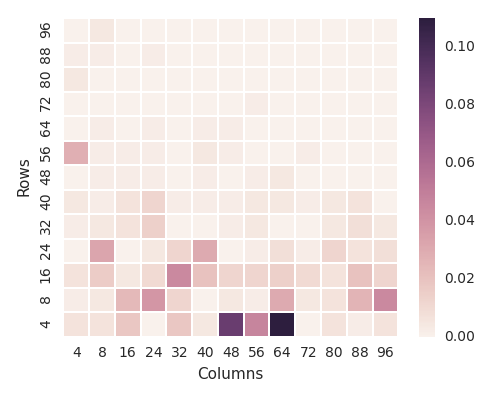
\includegraphics{gen/img/oracle_param_space.png}
\vspace{-1.5em} % Shrink vertical padding
\caption{Oracle workgroup sizes}
\label{fig:oracle-wgsizes}
\end{subfigure}
\caption{%
  On the left, the distribution of maximum legal workgroup sizes for
  all scenarios. On the right, the distribution of oracle workgroup
  sizes.%
}
\label{fig:heatmaps}
\end{figure}

\begin{figure}
\centering
\includegraphics{gen/img/num_params_oracle.png}
\caption{%
  Accuracy compared to the oracle as a function of the number of
  workgroup sizes used. The best accuracy that is achievable using a
  single statically chosen value is
  \protect\input{gen/max_oracle_param_frequency}\%.%
}
\label{fig:oracle-accuracy}
\end{figure}

\begin{figure}
\centering
\includegraphics{gen/img/performance_max_wgsize.png}
\caption{%
  Performance of a workgroup size relative to the oracle vs the
  maximum legal workgroup size. There is no clear trend between the
  performance of a workgroup size and it's size relative to the
  maximum allowed.%
}
\end{figure}

\begin{figure}
\centering
\includegraphics{gen/img/params_summary.png}
\caption{%
  The red line shows the ``legality'' of the parameter value, i.e.\
  the ratio of scenarios for which that workgroup size is legal.  The
  blue and green lines show the geometric mean of the performance of
  workgroup sizes relative to the oracle for: all scenarios, and only
  the scenarios for which the workgroup size is legal.%
}
\end{figure}



\section{Summary}
